\documentclass[compress, usepdftitle=false]{beamer}
\usepackage[utf8]{inputenc}
\usepackage[T1]{fontenc}
\usepackage{lmodern}
\usepackage[french]{babel}
\usepackage{amsfonts}
\usepackage{amsmath}
\usepackage{amsthm}

\useinnertheme{default}
\useoutertheme{miniframes}
\usecolortheme{beaver}
\usefonttheme[onlymath]{serif}
\setbeamercovered{transparent}
\setbeamertemplate{section in toc}[sections numbered]

\newcommand{\cont}{\mathcal{C}^0}
\newcommand{\cun}{\mathcal{C}^1}
\newcommand{\cinf}{\mathcal{C}^\infty}
\newcommand{\R}{\mathbb{R}}
\newcommand{\N}{\mathbb{N}}

\newtheorem{thm}{Théorème}
\newtheorem{cor}{Corollaire}
\newtheorem{lemm}{Lemme}
\theoremstyle{definition}
\newtheorem{defn}{Définition}

\author{Farid Arthaud}
\title{Théorie des catastrophes}
\subtitle{Supports visuels}
\date{}
\institute{TIPE ENS 2018}

\begin{document}
\frame{\titlepage}

\frame{\tableofcontents}

\section{Transversalité}
\begin{frame}{Intersection transverse en 2D}
    \begin{figure}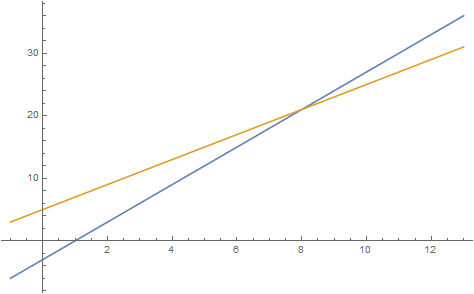
\includegraphics[keepaspectratio, height=0.8\textheight, width=\linewidth]{images/2DTransverse.png}\end{figure}
\end{frame}
\begin{frame}{Intersections transverses en 3D}
    \begin{figure}\includegraphics<1>[width=\linewidth, height=0.8\textheight, keepaspectratio]{images/3D_trans.png}
    \includegraphics<2>[width=\linewidth, height=0.8\textheight, keepaspectratio]{images/3D_non_trans.png}
    \includegraphics<3>[width=\linewidth, height=0.8\textheight, keepaspectratio]{images/var_trans.png}
    \includegraphics<4>[height=0.8\textheight,keepaspectratio]{images/saddle.png}
    \includegraphics<5>[width=\linewidth, height=0.8\textheight, keepaspectratio]{images/nontrans_rot9.png}
    \includegraphics<6>[width=\linewidth, height=0.8\textheight, keepaspectratio]{images/nontrans_rot13.png}
    \includegraphics<7>[width=\linewidth, height=0.8\textheight, keepaspectratio]{images/nontrans_rot17.png}
    \includegraphics<8>[width=\linewidth, height=0.8\textheight, keepaspectratio]{images/nontrans_rot19.png}
    \includegraphics<9>[width=\linewidth, height=0.8\textheight, keepaspectratio]{images/trans_fun.png}\end{figure}
\end{frame}

\section{Le pli et la fronce}
\begin{frame}{Le pli}
    \begin{figure}\includegraphics<1>[keepaspectratio, height=0.8\textheight, width=\linewidth]{images/fold_front.png}
    \includegraphics<2>[keepaspectratio, height=0.8\textheight, width=\linewidth]{images/fold_top.png}\end{figure}
\end{frame}
\begin{frame}{La fronce}
    \begin{figure}\includegraphics<1>[keepaspectratio, height=0.8\textheight, width=\linewidth]{images/cusp_front.png}
    \includegraphics<2>[keepaspectratio, height=0.8\textheight, width=\linewidth]{images/cusp_side.png}\end{figure}
\end{frame}

\section{Espace de germes}
\begin{frame}{Exponentielle}
    \alt<1>{$$\{(a,b,c) \mid b=c \} \subseteq J^1(\R,\R) \simeq \R^3$$}{$$j^1_x(exp) =  (x, e^x, e^x) \in \{(a,b,c) \mid b=c \}$$}

    \begin{figure}\includegraphics<1>[width=\linewidth, height=0.6\textheight, keepaspectratio]{images/equadiff.png}
    \includegraphics<2>[width=\linewidth, height=0.6\textheight, keepaspectratio]{images/exponential.png}\end{figure}
\end{frame}
\begin{frame}{$x\mapsto x^2$}
    \begin{figure}\includegraphics<1>[width=\linewidth, height=0.6\textheight, keepaspectratio]{images/x_deux_jet.png}\end{figure}
\end{frame}
\begin{frame}{Intersection non transverse}
    \begin{figure}\includegraphics<1>[width=\linewidth, height=0.6\textheight, keepaspectratio]{images/fun_non_jet.png}
    \includegraphics<2>[width=\linewidth, height=0.6\textheight, keepaspectratio]{images/fun_non_jet_deux.png}\end{figure}
\end{frame}

\section{Machine à catastrophes de \textsc{Zeeman}}
\begin{frame}{Montage physique}
    \begin{figure}\includegraphics<1>[keepaspectratio, height=0.8\textheight, width=\linewidth]{images/montage_loq.jpg}
    \includegraphics<2>[keepaspectratio, height=0.8\textheight, width=\linewidth]{images/eq_haut_loq.jpg}
    \includegraphics<3>[keepaspectratio, height=0.8\textheight, width=\linewidth]{images/eq_bas_loq.jpg}\end{figure}
\end{frame}
\begin{frame}{Analyse théorique}
    \begin{onlyenv}<2-3>
        $$E_p(a, b, x)  = \frac{1}{4}x^4+\frac{a}{2}x^2+bx + E_{p,0}$$

        \pause[3]
        \alert{Positions d'équilibre} ou points critiques:
        $$x^3+ax+b=0$$
    \end{onlyenv}
    \begin{figure}\includegraphics<1>[keepaspectratio, height=0.8\textheight, width=\linewidth]{images/zeeman_sketch.jpg}
    \includegraphics<4>[keepaspectratio, height=0.8\textheight, width=\linewidth]{images/cusp_zeeman.png}
    \includegraphics<5>[keepaspectratio, height=0.8\textheight, width=\linewidth]{images/cusp_zeeman_top.png}\end{figure}
\end{frame}

\end{document}
